\documentclass[12pt,a4paper]{report}

% ============================================================
% PACKAGES
% ============================================================
\usepackage[utf8]{inputenc}
\usepackage[T1]{fontenc}
\usepackage{lmodern}
\usepackage[margin=1in]{geometry}
\usepackage{graphicx}
\usepackage{xcolor}
\usepackage{hyperref}
\usepackage{listings}
\usepackage{amsmath,amssymb}
\usepackage{booktabs}
\usepackage{longtable}
\usepackage{float}
\usepackage{tikz}
\usetikzlibrary{shapes.geometric, arrows.meta, positioning, fit, calc}
\usepackage{fancyhdr}
\usepackage{tcolorbox}
\usepackage{enumitem}
\usepackage{caption}
\usepackage{subcaption}
\usepackage{array}

% ============================================================
% CONFIGURATION
% ============================================================
\hypersetup{
    colorlinks=true,
    linkcolor=blue!70!black,
    urlcolor=blue!60!black,
    citecolor=green!50!black,
    pdftitle={HippoVolume.AI - Comprehensive Technical Guide},
    pdfauthor={Student}
}

\lstset{
    basicstyle=\ttfamily\small,
    breaklines=true,
    frame=single,
    backgroundcolor=\color{gray!10},
    keywordstyle=\color{blue!70!black}\bfseries,
    commentstyle=\color{green!50!black},
    stringstyle=\color{red!60!black},
    numbers=left,
    numberstyle=\tiny\color{gray},
    numbersep=5pt,
    tabsize=4,
    showspaces=false,
    showstringspaces=false
}

\tcbuselibrary{skins,breakable}

\newtcolorbox{conceptbox}[1]{
    colback=blue!5!white,
    colframe=blue!60!black,
    fonttitle=\bfseries,
    title=#1,
    breakable
}

\newtcolorbox{warningbox}[1]{
    colback=red!5!white,
    colframe=red!60!black,
    fonttitle=\bfseries,
    title=#1,
    breakable
}

\newtcolorbox{infobox}[1]{
    colback=green!5!white,
    colframe=green!60!black,
    fonttitle=\bfseries,
    title=#1,
    breakable
}

\pagestyle{fancy}
\fancyhf{}
\fancyhead[L]{\leftmark}
\fancyhead[R]{HippoVolume.AI}
\fancyfoot[C]{\thepage}

% ============================================================
% DOCUMENT
% ============================================================
\begin{document}

% ============================================================
% TITLE PAGE
% ============================================================
\begin{titlepage}
\centering
\vspace*{2cm}
{\Huge\bfseries HippoVolume.AI\\[0.5cm]}
{\LARGE Comprehensive Technical Guide\\[0.3cm]}
{\Large Hippocampal Volume Quantification\\Using Deep Learning\\[2cm]}
\rule{\textwidth}{1pt}\\[1cm]
{\large An End-to-End Guide to Understanding\\
3D Medical Image Segmentation for Alzheimer's Disease Tracking\\[2cm]}
{\large Udacity AI for Healthcare Nanodegree\\
Course 3: 3D Medical Imaging\\[1cm]}
{\large Date: March 8, 2026}
\vfill
\end{titlepage}

\tableofcontents
\newpage

% ============================================================
% CHAPTER 1: INTRODUCTION & BACKGROUND
% ============================================================
\chapter{Introduction and Background}

\section{What Is This Project About?}

This project builds a complete \textbf{AI-powered clinical system} that automatically measures the volume of the \textbf{hippocampus} from brain MRI scans. The hippocampus is a critical brain structure involved in memory formation, and its shrinkage (atrophy) is one of the earliest biomarkers of \textbf{Alzheimer's disease}.

\begin{conceptbox}{Why Hippocampal Volume Matters}
\begin{itemize}
    \item The hippocampus is located in the medial temporal lobe of the brain
    \item Normal adult hippocampal volume: approximately \textbf{2,500--4,500 mm\textsuperscript{3}} per side
    \item In Alzheimer's disease, the hippocampus can lose \textbf{10--25\%} of its volume per year
    \item Manual segmentation by a radiologist takes \textbf{30--60 minutes} per scan
    \item Our AI system does it in \textbf{under 5 seconds}
\end{itemize}
\end{conceptbox}

\section{Project Architecture Overview}

The project is divided into three major sections, each representing a stage in a real-world clinical AI pipeline:

\begin{enumerate}
    \item \textbf{Section 1: Data Exploration \& Curation} --- Understand and clean the medical imaging dataset
    \item \textbf{Section 2: Machine Learning Pipeline} --- Train a U-Net deep learning model for segmentation
    \item \textbf{Section 3: Clinical Deployment} --- Integrate the model into a hospital PACS system
\end{enumerate}

\section{Full System Architecture Diagram}

\begin{figure}[H]
\centering
\begin{tikzpicture}[
    node distance=1.2cm and 2cm,
    box/.style={rectangle, draw, rounded corners, minimum width=3.5cm, minimum height=1cm, text centered, font=\small},
    data/.style={box, fill=blue!15},
    process/.style={box, fill=orange!15},
    model/.style={box, fill=green!15},
    output/.style={box, fill=red!15},
    arrow/.style={-{Stealth[length=3mm]}, thick},
    dashedarrow/.style={-{Stealth[length=3mm]}, thick, dashed}
]

% Section 1
\node[data] (nifti) {NIFTI Volumes\\(394 images)};
\node[process, below=of nifti] (eda) {EDA \& Cleaning\\(Section 1)};
\node[data, below=of eda] (clean) {Clean Dataset\\(260 volumes)};

% Section 2
\node[process, below=of clean] (loader) {Data Loader\\HippocampusDatasetLoader};
\node[process, below=of loader] (slices) {2D Slice Extraction\\SlicesDataset (9,198 slices)};
\node[model, below=of slices] (unet) {U-Net Model\\(Recursive, 3-class)};
\node[process, below=of unet] (training) {Training Loop\\(10 epochs, Adam)};
\node[output, below=of training] (modelpth) {Trained Model\\(model.pth)};

% Section 3
\node[data, right=3cm of nifti] (mri) {MRI Scanner};
\node[process, below=of mri] (pacs) {Orthanc PACS\\(Port 4242)};
\node[process, below=of pacs] (routing) {Lua Auto-Routing\\Script};
\node[process, below=of routing] (listener) {storescp Listener\\(Port 106)};
\node[process, below=of listener] (infdcm) {inference\_dcm.py};
\node[model, below=of infdcm] (inference) {U-Net Inference\\Agent (CPU)};
\node[output, below=of inference] (report) {DICOM Report\\(1000$\times$1000 RGB)};
\node[process, below=of report] (storescu) {storescu\\(Send back to PACS)};

% Arrows Section 1-2
\draw[arrow] (nifti) -- (eda);
\draw[arrow] (eda) -- (clean);
\draw[arrow] (clean) -- (loader);
\draw[arrow] (loader) -- (slices);
\draw[arrow] (slices) -- (unet);
\draw[arrow] (unet) -- (training);
\draw[arrow] (training) -- (modelpth);

% Arrows Section 3
\draw[arrow] (mri) -- (pacs);
\draw[arrow] (pacs) -- (routing);
\draw[arrow] (routing) -- (listener);
\draw[arrow] (listener) -- (infdcm);
\draw[arrow] (infdcm) -- (inference);
\draw[arrow] (inference) -- (report);
\draw[arrow] (report) -- (storescu);
\draw[arrow] (storescu.south) -- ++(0,-0.5) -| ($(pacs.east)+(0.5,0)$) -- (pacs.east);

% Cross connection
\draw[dashedarrow] (modelpth.east) -- ++(1,0) |- (inference.west);

% Labels
\node[above=0.3cm of nifti, font=\large\bfseries, color=blue!70!black] {TRAINING PIPELINE};
\node[above=0.3cm of mri, font=\large\bfseries, color=red!70!black] {CLINICAL PIPELINE};

% Bounding boxes
\begin{scope}[on background layer]
\node[fit=(nifti)(eda)(clean), draw=blue!40, fill=blue!3, rounded corners, inner sep=10pt, label={[font=\small\bfseries, color=blue!60]above left:Section 1}] {};
\node[fit=(loader)(slices)(unet)(training)(modelpth), draw=orange!40, fill=orange!3, rounded corners, inner sep=10pt, label={[font=\small\bfseries, color=orange!60]above left:Section 2}] {};
\node[fit=(mri)(pacs)(routing)(listener)(infdcm)(inference)(report)(storescu), draw=red!40, fill=red!3, rounded corners, inner sep=10pt, label={[font=\small\bfseries, color=red!60]above right:Section 3}] {};
\end{scope}

\end{tikzpicture}
\caption{Full System Architecture --- Training Pipeline (left) and Clinical Deployment Pipeline (right). The dashed arrow shows the trained model being loaded into the inference agent.}
\label{fig:full-architecture}
\end{figure}


% ============================================================
% CHAPTER 2: THE DATASET
% ============================================================
\chapter{Understanding the Dataset}

\section{Medical Imaging Formats}

\begin{conceptbox}{NIFTI vs DICOM}
\begin{itemize}
    \item \textbf{NIFTI} (Neuroimaging Informatics Technology Initiative): Used in research. A single \texttt{.nii.gz} file stores the entire 3D volume. Simple header with spatial metadata.
    \item \textbf{DICOM} (Digital Imaging and Communications in Medicine): Used in hospitals. Each 2D slice is a separate \texttt{.dcm} file. Rich metadata (patient info, scanner settings, etc.).
    \item Section 1--2 uses NIFTI; Section 3 uses DICOM --- mirroring real-world research-to-clinic transition.
\end{itemize}
\end{conceptbox}

\section{Dataset Structure}

\subsection{Training Set}
\begin{itemize}
    \item \textbf{Location}: \texttt{data/TrainingSet/}
    \item \textbf{Format}: NIFTI (\texttt{.nii.gz} compressed)
    \item \textbf{Total volumes}: 260 clean volumes (after EDA filtering)
    \item \textbf{Resolution}: $1 \times 1 \times 1$ mm voxel spacing (isotropic)
    \item Contains two subdirectories:
    \begin{itemize}
        \item \texttt{images/} --- MRI intensity volumes (e.g., \texttt{hippocampus\_001.nii.gz})
        \item \texttt{labels/} --- Corresponding segmentation masks (same filenames)
    \end{itemize}
\end{itemize}

\subsection{Label Classes}
The segmentation masks contain three classes:

\begin{table}[H]
\centering
\begin{tabular}{cll}
\toprule
\textbf{Value} & \textbf{Class} & \textbf{Description} \\
\midrule
0 & Background & Non-hippocampal tissue \\
1 & Anterior Hippocampus & Head of the hippocampus \\
2 & Posterior Hippocampus & Body and tail of the hippocampus \\
\bottomrule
\end{tabular}
\caption{Segmentation label classes}
\end{table}

\subsection{Test Volumes (Section 3)}
\begin{itemize}
    \item \textbf{Location}: \texttt{data/TestVolumes/}
    \item \textbf{Format}: DICOM (one \texttt{.dcm} file per slice)
    \item Contains 3 complete brain studies (Study1, Study2, Study3)
    \item Each study has multiple series (T1post, FLAIR, T2, HippoCrop, etc.)
    \item Only the \textbf{HippoCrop} series is used for inference
\end{itemize}

\section{Exploratory Data Analysis (Section 1)}

The Jupyter notebook (\texttt{section1/Final Project EDA.ipynb}) performs:

\begin{enumerate}
    \item \textbf{Loading}: Uses \texttt{nibabel} to read NIFTI files
    \item \textbf{Visualization}: Displays axial, coronal, and sagittal slices
    \item \textbf{Statistics}: Computes voxel intensity distributions, volume sizes
    \item \textbf{Quality check}: Identifies and removes mismatched/corrupted pairs
    \item \textbf{Volume calculation}: Validates hippocampal volumes against clinical reference ranges (2,200--4,500 mm\textsuperscript{3})
    \item \textbf{Output}: Copies clean, validated volumes to \texttt{section1/out/} for training
\end{enumerate}

\begin{warningbox}{Key Finding: Missing Data}
File \texttt{hippocampus\_118.nii.gz} exists in the images directory but has no corresponding label --- it was excluded from the training set.
\end{warningbox}


% ============================================================
% CHAPTER 3: U-NET ARCHITECTURE
% ============================================================
\chapter{U-Net Architecture Deep Dive}

\section{What Is U-Net?}

U-Net is a \textbf{fully convolutional neural network} designed specifically for biomedical image segmentation. It was introduced by Ronneberger et al.\ in 2015 and has become the \textit{de facto} standard for medical image segmentation.

\begin{conceptbox}{Key Innovation of U-Net}
U-Net's distinguishing feature is its \textbf{skip connections} (also called ``shortcut connections''). These connections bridge the encoding (downsampling) path with the decoding (upsampling) path, allowing the network to combine:
\begin{itemize}
    \item \textbf{High-level semantic features} (what is this?) from deep layers
    \item \textbf{Fine-grained spatial details} (where exactly?) from shallow layers
\end{itemize}
This is critical for segmentation, where you need both understanding of what a structure is AND precise boundary localization.
\end{conceptbox}

\section{Our Specific Implementation: Recursive U-Net}

We use a \textbf{recursive implementation} from the German Cancer Research Center (DKFZ). Instead of building the entire network layer by layer, it constructs the U-shape recursively:

\subsection{Architecture Parameters}

\begin{table}[H]
\centering
\begin{tabular}{ll}
\toprule
\textbf{Parameter} & \textbf{Value} \\
\midrule
Input channels & 1 (grayscale MRI) \\
Output classes & 3 (background, anterior, posterior) \\
Initial filter size & 64 \\
Number of downsampling levels & 4 \\
Normalization & Instance Normalization \\
Activation & LeakyReLU \\
Final layer & $1 \times 1$ Convolution \\
Approximate parameters & $\sim$31 million \\
\bottomrule
\end{tabular}
\end{table}

\subsection{Architecture Diagram}

\begin{figure}[H]
\centering
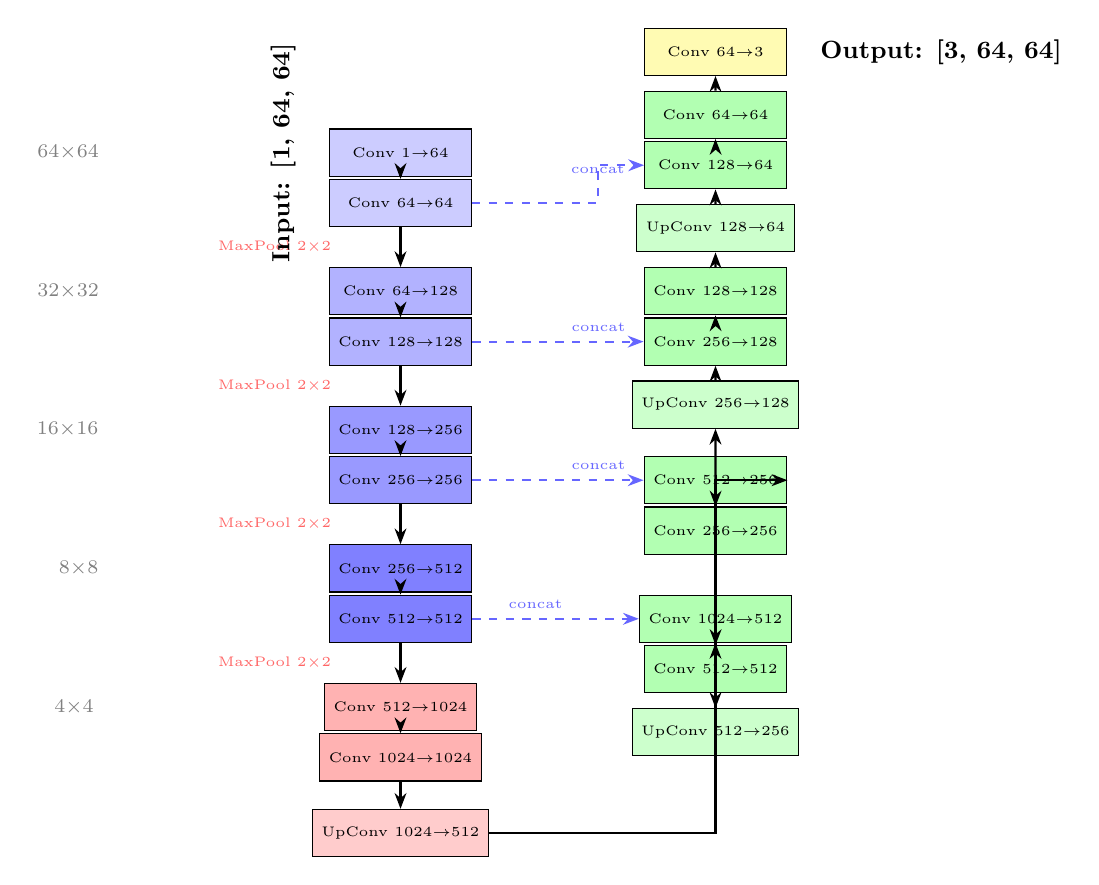
\begin{tikzpicture}[
    scale=0.8,
    block/.style={rectangle, draw, fill=#1, minimum width=1.8cm, minimum height=0.6cm, text centered, font=\tiny},
    arrow/.style={-{Stealth[length=2mm]}, thick},
    skip/.style={-{Stealth[length=2mm]}, thick, blue!60, dashed}
]

% Encoder path (left side)
\node[block=blue!20] (e1) at (0,0) {Conv 1$\to$64};
\node[block=blue!20] (e1b) at (0,-0.8) {Conv 64$\to$64};

\node[block=blue!30] (e2) at (0,-2.2) {Conv 64$\to$128};
\node[block=blue!30] (e2b) at (0,-3.0) {Conv 128$\to$128};

\node[block=blue!40] (e3) at (0,-4.4) {Conv 128$\to$256};
\node[block=blue!40] (e3b) at (0,-5.2) {Conv 256$\to$256};

\node[block=blue!50] (e4) at (0,-6.6) {Conv 256$\to$512};
\node[block=blue!50] (e4b) at (0,-7.4) {Conv 512$\to$512};

% Bottleneck
\node[block=red!30] (bn1) at (0,-8.8) {Conv 512$\to$1024};
\node[block=red!30] (bn2) at (0,-9.6) {Conv 1024$\to$1024};

% Up path
\node[block=red!20] (up4) at (0,-10.8) {UpConv 1024$\to$512};

% Decoder path (right side)
\node[block=green!30] (d4) at (5,-7.4) {Conv 1024$\to$512};
\node[block=green!30] (d4b) at (5,-8.2) {Conv 512$\to$512};
\node[block=green!20] (up3) at (5,-9.2) {UpConv 512$\to$256};

\node[block=green!30] (d3) at (5,-5.2) {Conv 512$\to$256};
\node[block=green!30] (d3b) at (5,-6.0) {Conv 256$\to$256};
\node[block=green!20] (up2) at (5,-4.0) {UpConv 256$\to$128};

\node[block=green!30] (d2) at (5,-3.0) {Conv 256$\to$128};
\node[block=green!30] (d2b) at (5,-2.2) {Conv 128$\to$128};
\node[block=green!20] (up1) at (5,-1.2) {UpConv 128$\to$64};

\node[block=green!30] (d1) at (5,-0.2) {Conv 128$\to$64};
\node[block=green!30] (d1b) at (5,0.6) {Conv 64$\to$64};
\node[block=yellow!30] (final) at (5,1.6) {Conv 64$\to$3};

% Pooling operations
\node[font=\tiny, color=red!60] at (-2.0,-1.5) {MaxPool 2$\times$2};
\node[font=\tiny, color=red!60] at (-2.0,-3.7) {MaxPool 2$\times$2};
\node[font=\tiny, color=red!60] at (-2.0,-5.9) {MaxPool 2$\times$2};
\node[font=\tiny, color=red!60] at (-2.0,-8.1) {MaxPool 2$\times$2};

% Encoder arrows
\draw[arrow] (e1) -- (e1b);
\draw[arrow] (e1b) -- node[left, font=\tiny] {} (e2);
\draw[arrow] (e2) -- (e2b);
\draw[arrow] (e2b) -- (e3);
\draw[arrow] (e3) -- (e3b);
\draw[arrow] (e3b) -- (e4);
\draw[arrow] (e4) -- (e4b);
\draw[arrow] (e4b) -- (bn1);
\draw[arrow] (bn1) -- (bn2);
\draw[arrow] (bn2) -- (up4);

% Skip connections
\draw[skip] (e4b.east) -- ++(1,0) |- (d4.west) node[pos=0.25, above, font=\tiny, blue!60] {concat};
\draw[skip] (e3b.east) -- ++(2,0) |- (d3.west) node[pos=0.25, above, font=\tiny, blue!60] {concat};
\draw[skip] (e2b.east) -- ++(2,0) |- (d2.west) node[pos=0.25, above, font=\tiny, blue!60] {concat};
\draw[skip] (e1b.east) -- ++(2,0) |- (d1.west) node[pos=0.25, above, font=\tiny, blue!60] {concat};

% Decoder arrows
\draw[arrow] (up4.east) -| (d4.south);
\draw[arrow] (d4) -- (d4b);
\draw[arrow] (d4b) -- (up3);
\draw[arrow] (up3.north) |- (d3.east);
\draw[arrow] (d3) -- (d3b);
\draw[arrow] (d3b) -- (up2);
\draw[arrow] (up2) -- (d2);
\draw[arrow] (d2) -- (d2b);
\draw[arrow] (d2b) -- (up1);
\draw[arrow] (up1) -- (d1);
\draw[arrow] (d1) -- (d1b);
\draw[arrow] (d1b) -- (final);

% Labels
\node[left=0.3cm of e1, font=\small\bfseries, rotate=90, anchor=south] {Input: [1, 64, 64]};
\node[right=0.3cm of final, font=\small\bfseries] {Output: [3, 64, 64]};

% Size annotations
\node[left=2.8cm of e1, font=\scriptsize, color=gray] {64$\times$64};
\node[left=2.8cm of e2, font=\scriptsize, color=gray] {32$\times$32};
\node[left=2.8cm of e3, font=\scriptsize, color=gray] {16$\times$16};
\node[left=2.8cm of e4, font=\scriptsize, color=gray] {8$\times$8};
\node[left=2.8cm of bn1, font=\scriptsize, color=gray] {4$\times$4};

\end{tikzpicture}
\caption{Recursive U-Net architecture used in this project. Blue dashed lines are skip connections. Each encoder level halves spatial dimensions while doubling feature channels.}
\label{fig:unet-arch}
\end{figure}

\subsection{Detailed Layer-by-Layer Walkthrough}

\subsubsection{Encoder (Contracting Path)}

Each encoder level consists of:
\begin{enumerate}
    \item \textbf{MaxPool2d}$(2 \times 2)$: Halves spatial dimensions (except the outermost level)
    \item \textbf{Conv2d}$(k=3, p=1)$: $3 \times 3$ convolution with padding to preserve size
    \item \textbf{InstanceNorm2d}: Normalizes each feature map independently (better than BatchNorm for small batches)
    \item \textbf{LeakyReLU}: Activation function ($\alpha = 0.01$ negative slope)
    \item Repeat conv $\to$ norm $\to$ activation once more
\end{enumerate}

Spatial dimensions at each level for a $64 \times 64$ input:
$$64 \times 64 \xrightarrow{\text{pool}} 32 \times 32 \xrightarrow{\text{pool}} 16 \times 16 \xrightarrow{\text{pool}} 8 \times 8 \xrightarrow{\text{pool}} 4 \times 4$$

\subsubsection{Bottleneck}
At the bottom of the ``U'', we have the deepest representation at $4 \times 4$ with 1024 channels. This is the most abstract, semantically rich representation of the input.

\subsubsection{Decoder (Expanding Path)}
Each decoder level:
\begin{enumerate}
    \item \textbf{ConvTranspose2d}$(k=2, s=2)$: Upsamples by $2\times$ (``learnable upsampling'')
    \item \textbf{Concatenation}: Skip connection combines decoder features with corresponding encoder features (channel-wise)
    \item \textbf{Center crop}: Aligns spatial dimensions before concatenation
    \item Two conv $\to$ LeakyReLU blocks to process the concatenated features
\end{enumerate}

\subsubsection{Output Layer}
A $1 \times 1$ convolution maps from 64 channels to 3 channels (one per class). No activation --- raw logits are output, and softmax is applied during loss computation.

\section{Why Instance Normalization?}

\begin{conceptbox}{Instance Norm vs Batch Norm}
\begin{itemize}
    \item \textbf{Batch Normalization}: Normalizes across the entire batch. Works well with large batches ($\geq 32$). Statistics become noisy with small batches.
    \item \textbf{Instance Normalization}: Normalizes each sample independently. Works well regardless of batch size. Better for medical imaging where intensity distributions vary between patients/scanners.
\end{itemize}
Since we use batch size 8, Instance Norm is the better choice.
\end{conceptbox}


% ============================================================
% CHAPTER 4: DATA PIPELINE
% ============================================================
\chapter{Data Pipeline in Detail}

\section{Overview}

The data pipeline transforms raw NIFTI volumes into PyTorch tensors suitable for training:

$$\text{NIFTI files} \xrightarrow{\text{Load}} \text{3D volumes} \xrightarrow{\text{Normalize}} [0,1] \xrightarrow{\text{Reshape}} 64 \times 64 \xrightarrow{\text{Slice}} \text{2D tensors} \xrightarrow{\text{Batch}} \text{DataLoader}$$

\section{Step 1: Loading (HippocampusDatasetLoader.py)}

\begin{lstlisting}[language=Python, caption=Image Loading and Normalization]
image, _ = load(os.path.join(image_dir, f))
label, _ = load(os.path.join(label_dir, f))

# Normalize images to [0, 1]
image = image.astype(np.float64)
if image.max() > 0:
    image = image / image.max()

# Reshape to consistent patch size
image = med_reshape(image, new_shape=(image.shape[0], 64, 64))
label = med_reshape(label, new_shape=(label.shape[0], 64, 64)).astype(int)
\end{lstlisting}

\begin{conceptbox}{Why Normalize to [0, 1]?}
\begin{itemize}
    \item MRI intensities are arbitrary --- different scanners produce different ranges
    \item Neural networks train faster and more stably with normalized inputs
    \item Divide by \texttt{image.max()} performs min-max normalization (min is assumed to be 0 for MRI)
    \item Labels are NOT normalized --- they contain class indices (0, 1, 2)
\end{itemize}
\end{conceptbox}

\subsection{The med\_reshape Function}

\begin{lstlisting}[language=Python, caption=Zero-padding reshape function]
def med_reshape(image, new_shape):
    reshaped_image = np.zeros(new_shape)
    reshaped_image[:min(image.shape[0], new_shape[0]),
                   :min(image.shape[1], new_shape[1]),
                   :min(image.shape[2], new_shape[2])] = \
        image[:min(image.shape[0], new_shape[0]),
              :min(image.shape[1], new_shape[1]),
              :min(image.shape[2], new_shape[2])]
    return reshaped_image
\end{lstlisting}

This function pads the volume with zeros to reach the target size $64 \times 64$ (coronal and sagittal dimensions), keeping the axial dimension unchanged. The original data is placed in the top-left corner.

\section{Step 2: 2D Slicing (SlicesDataset.py)}

Since we use a \textbf{2D U-Net}, we cannot feed 3D volumes directly. Instead, we extract individual 2D axial slices:

\begin{lstlisting}[language=Python, caption=Creating indexable slice dataset]
class SlicesDataset(Dataset):
    def __init__(self, data):
        self.data = data
        self.slices = []
        for i, d in enumerate(data):
            for j in range(d["image"].shape[0]):
                self.slices.append((i, j))  # (volume_idx, slice_idx)
\end{lstlisting}

Each index in the dataset maps to a tuple \texttt{(volume\_index, slice\_number)}.

\textbf{Total slices}: 260 volumes $\times$ ~35 slices/volume $\approx$ 9,198 slices

\subsection{Tensor Shape}

Each sample returned by \texttt{\_\_getitem\_\_} has shape:
$$\text{image}: [1, 64, 64] \quad \text{seg}: [1, 64, 64]$$

The leading dimension of size 1 is the \textbf{channel dimension} (grayscale = 1 channel). When batched by DataLoader with batch size 8:
$$\text{batch}: [8, 1, 64, 64]$$

\section{Step 3: Train/Val/Test Split}

\begin{lstlisting}[language=Python, caption=Data split (70/10/20)]
total = len(keys)  # 260
train_end = int(0.7 * total)   # 182
val_end = int(0.8 * total)      # 208

split["train"] = list(range(0, 182))     # 182 volumes
split["val"]   = list(range(182, 208))   # 26 volumes  
split["test"]  = list(range(208, 260))   # 52 volumes
\end{lstlisting}

\begin{warningbox}{Important: Volume-Level Split}
The split is done at the \textbf{volume level}, not the slice level. This prevents data leakage --- slices from the same patient never appear in both training and testing sets.
\end{warningbox}


% ============================================================
% CHAPTER 5: TRAINING PROCESS
% ============================================================
\chapter{Training Process}

\section{Training Configuration}

\begin{table}[H]
\centering
\begin{tabular}{ll}
\toprule
\textbf{Hyperparameter} & \textbf{Value} \\
\midrule
Number of epochs & 10 \\
Batch size & 8 \\
Learning rate & 0.0002 \\
Optimizer & Adam ($\beta_1=0.9, \beta_2=0.999$) \\
Loss function & CrossEntropyLoss \\
LR scheduler & ReduceLROnPlateau \\
Device & CUDA (GPU) if available, else CPU \\
\bottomrule
\end{tabular}
\caption{Training hyperparameters}
\end{table}

\section{Loss Function: Cross-Entropy}

The \textbf{Cross-Entropy Loss} for multi-class segmentation is:

$$\mathcal{L} = -\frac{1}{N} \sum_{i=1}^{N} \sum_{c=0}^{C-1} y_{i,c} \log(p_{i,c})$$

where:
\begin{itemize}
    \item $N$ = total number of pixels per batch
    \item $C$ = 3 (number of classes)
    \item $y_{i,c}$ = 1 if pixel $i$ belongs to class $c$, 0 otherwise
    \item $p_{i,c}$ = predicted probability for pixel $i$ being class $c$ (softmax output)
\end{itemize}

\begin{conceptbox}{Why Cross-Entropy and Not Dice Loss?}
Cross-Entropy is a pixel-wise loss that treats each pixel independently. It's a good starting point and provides stable gradients. Dice Loss could be used as a complement --- it directly optimizes the evaluation metric (Dice coefficient) and handles class imbalance better.
\end{conceptbox}

\section{Training Loop}

\begin{lstlisting}[language=Python, caption=Core training step]
for i, batch in enumerate(self.train_loader):
    self.optimizer.zero_grad()
    
    data = batch["image"].to(device, dtype=torch.float)      # [B, 1, 64, 64]
    target = batch["seg"].to(device, dtype=torch.long)        # [B, 1, 64, 64]
    
    prediction = self.model(data)                             # [B, 3, 64, 64]
    loss = self.loss_function(prediction, target[:, 0, :, :]) # target: [B, 64, 64]
    
    loss.backward()
    self.optimizer.step()
\end{lstlisting}

\subsection{Tensor Dimensions Explained}

\begin{table}[H]
\centering
\begin{tabular}{lll}
\toprule
\textbf{Variable} & \textbf{Shape} & \textbf{Meaning} \\
\midrule
\texttt{data} & $[B, 1, 64, 64]$ & Batch, Channel, Height, Width \\
\texttt{target} & $[B, 1, 64, 64]$ & Batch, Channel, Height, Width (class indices) \\
\texttt{prediction} & $[B, 3, 64, 64]$ & Batch, Classes, Height, Width (logits) \\
\texttt{target[:,0,:,:]} & $[B, 64, 64]$ & Remove channel dim (CE expects this) \\
\bottomrule
\end{tabular}
\end{table}

\section{Learning Rate Scheduling}

\texttt{ReduceLROnPlateau} monitors the validation loss. When it stops decreasing (``plateaus''), the learning rate is automatically reduced:

$$\text{lr}_{\text{new}} = \text{lr}_{\text{old}} \times \text{factor}$$

This prevents the optimizer from oscillating around a minimum by taking smaller steps.

\section{TensorBoard Monitoring}

The training logs are written to the \texttt{runs/} directory and can be visualized with:
\begin{lstlisting}[language=bash]
tensorboard --logdir section2/src/runs/
\end{lstlisting}

Logged metrics include: loss curves, input images, ground truth masks, softmax probability maps, and argmax predictions.

\section{Training Results}

\begin{table}[H]
\centering
\begin{tabular}{ccc}
\toprule
\textbf{Epoch} & \textbf{Last Batch Train Loss} & \textbf{Trend} \\
\midrule
0 & 0.024468 & --- \\
1 & 0.013140 & $\downarrow$ \\
2 & 0.018062 & $\uparrow$ (fluctuation) \\
3 & 0.008420 & $\downarrow$ \\
4 & 0.022230 & $\uparrow$ \\
5 & 0.013507 & $\downarrow$ \\
6 & 0.004962 & $\downarrow$ \\
7 & 0.007267 & $\uparrow$ (minor) \\
8 & 0.007769 & stable \\
9 & 0.008651 & stable \\
\bottomrule
\end{tabular}
\caption{Training loss progression over 10 epochs. Total training time: 12 minutes 18 seconds.}
\end{table}


% ============================================================
% CHAPTER 6: EVALUATION METRICS
% ============================================================
\chapter{Evaluation Metrics}

\section{Why These Metrics?}

Medical image segmentation requires specialized metrics that assess the overlap between predicted and ground truth volumes.

\section{Dice Similarity Coefficient (DSC)}

The Dice coefficient measures the overlap between two binary volumes:

$$\text{DSC} = \frac{2|A \cap B|}{|A| + |B|}$$

\begin{itemize}
    \item Range: 0 (no overlap) to 1 (perfect overlap)
    \item Returns $-1$ when both volumes are empty
    \item \textbf{Our result: Mean DSC = 0.9001}
\end{itemize}

\begin{lstlisting}[language=Python, caption=Dice3d implementation]
def Dice3d(a, b):
    a_binary = (a > 0).astype(int)
    b_binary = (b > 0).astype(int)
    intersection = np.sum(a_binary * b_binary)
    volumes = np.sum(a_binary) + np.sum(b_binary)
    if volumes == 0:
        return -1
    return 2.0 * intersection / volumes
\end{lstlisting}

\section{Jaccard Index (IoU)}

Also known as Intersection over Union:

$$J = \frac{|A \cap B|}{|A \cup B|} = \frac{|A \cap B|}{|A| + |B| - |A \cap B|}$$

\begin{itemize}
    \item Range: 0 to 1
    \item More intuitive geometric interpretation than Dice
    \item Related to Dice: $J = \frac{D}{2-D}$
    \item \textbf{Our result: Mean Jaccard = 0.8195}
\end{itemize}

\section{Sensitivity (Recall / True Positive Rate)}

$$\text{Sensitivity} = \frac{TP}{TP + FN}$$

\begin{itemize}
    \item Measures what fraction of the real hippocampus was correctly identified
    \item Low sensitivity $\Rightarrow$ under-segmentation (missing hippocampal tissue)
    \item Critical in clinical context: missing a shrunken hippocampus could mean missing Alzheimer's
\end{itemize}

\section{Specificity (True Negative Rate)}

$$\text{Specificity} = \frac{TN}{TN + FP}$$

\begin{itemize}
    \item Measures how well the model avoids false positives
    \item Low specificity $\Rightarrow$ over-segmentation (labeling non-hippocampus as hippocampus)
    \item Typically very high in our case ($>0.99$) because background vastly outnumbers hippocampus
\end{itemize}

\section{Per-Class Dice Score}

Computes Dice separately for anterior (class 1) and posterior (class 2):
$$\text{Dice}_{c} = \frac{2 \sum_i \mathbb{1}[P_i = c] \cdot \mathbb{1}[G_i = c]}{\sum_i \mathbb{1}[P_i = c] + \sum_i \mathbb{1}[G_i = c]}$$

\section{Test Results Summary}

\begin{table}[H]
\centering
\begin{tabular}{lc}
\toprule
\textbf{Metric} & \textbf{Value} \\
\midrule
Mean Dice & 0.9001 \\
Std Dice & --- \\
Best Dice & 0.9368 (\texttt{hippocampus\_146.nii.gz}) \\
Worst Dice & 0.8229 (\texttt{hippocampus\_334.nii.gz}) \\
Mean Jaccard & 0.8195 \\
Mean Sensitivity & $\sim$0.89 \\
Mean Specificity & $\sim$0.998 \\
\bottomrule
\end{tabular}
\caption{Overall test set performance on 52 test volumes}
\end{table}

\begin{infobox}{Interpreting the Results}
\begin{itemize}
    \item A mean Dice of \textbf{0.90} is considered \textbf{excellent} for hippocampal segmentation
    \item The narrow range (0.82--0.94) shows consistent performance across patients
    \item High specificity ($>0.99$) means the model rarely marks non-hippocampal tissue
    \item The small gap between sensitivity ($\sim$0.89) and Dice ($\sim$0.90) suggests balanced over/under-segmentation
\end{itemize}
\end{infobox}


% ============================================================
% CHAPTER 7: INFERENCE PIPELINE
% ============================================================
\chapter{Inference Pipeline}

\section{Section 2 Inference Agent}

The \texttt{UNetInferenceAgent} class handles prediction on full 3D volumes:

\begin{lstlisting}[language=Python, caption=Slice-by-slice inference]
def single_volume_inference(self, volume):
    self.model.eval()
    slices = np.zeros(volume.shape)
    
    for slc_ix in range(volume.shape[0]):
        slc = volume[slc_ix, :, :]
        slc_tensor = torch.from_numpy(slc[None, None, :, :]).float()
        prediction = self.model(slc_tensor)
        pred_label = torch.argmax(prediction, dim=1).squeeze().cpu().numpy()
        slices[slc_ix, :, :] = pred_label
    
    return slices
\end{lstlisting}

\subsection{How It Works}
\begin{enumerate}
    \item Takes a 3D volume of shape $[X, 64, 64]$
    \item Loops through each axial slice along dimension 0
    \item Adds batch and channel dimensions: $[64, 64] \to [1, 1, 64, 64]$
    \item Feeds through the model to get $[1, 3, 64, 64]$ (3-class logits)
    \item Takes \texttt{argmax} along class dimension to get the predicted label
    \item Assembles all slices into a 3D prediction mask
\end{enumerate}

\section{Section 3 Inference Agent (Unpadded)}

For clinical deployment, volumes may not be exactly $64 \times 64$. The unpadded version handles arbitrary sizes:

\begin{lstlisting}[language=Python, caption=Inference with automatic padding/cropping]
def single_volume_inference_unpadded(self, volume):
    orig_shape = volume.shape
    
    # Pad to 64x64
    new_shape = (orig_shape[0], self.patch_size, self.patch_size)
    padded_volume = np.zeros(new_shape)
    padded_volume[:orig_shape[0], :orig_shape[1], :orig_shape[2]] = volume
    
    # Run inference on padded volume
    prediction = np.zeros(new_shape)
    for slc_ix in range(padded_volume.shape[0]):
        slc = padded_volume[slc_ix, :, :]
        slc_tensor = torch.from_numpy(slc[None, None, :, :]).float()
        with torch.no_grad():
            output = self.model(slc_tensor)
        pred_label = torch.argmax(output, dim=1).squeeze().cpu().numpy()
        prediction[slc_ix, :, :] = pred_label
    
    # Crop back to original size
    return prediction[:orig_shape[0], :orig_shape[1], :orig_shape[2]]
\end{lstlisting}


% ============================================================
% CHAPTER 8: CLINICAL DEPLOYMENT
% ============================================================
\chapter{Clinical Deployment (Section 3)}

\section{DICOM and PACS Overview}

\begin{conceptbox}{What is PACS?}
\textbf{PACS} (Picture Archiving and Communication System) is the standard hospital infrastructure for storing and distributing medical images. All modern hospitals use PACS. Key concepts:
\begin{itemize}
    \item \textbf{DICOM}: The universal format for medical images (like JPEG for photos)
    \item \textbf{Orthanc}: Our open-source PACS server (lightweight, free)
    \item \textbf{OHIF}: Web-based DICOM viewer (like the radiologist's screen)
    \item \textbf{DIMSE}: The network protocol for sending/receiving DICOM files
    \item \textbf{C-STORE}: A DIMSE command for sending (storing) images
    \item \textbf{AET}: Application Entity Title --- like a ``name'' for network nodes
\end{itemize}
\end{conceptbox}

\section{Clinical Deployment Architecture}

\begin{figure}[H]
\centering
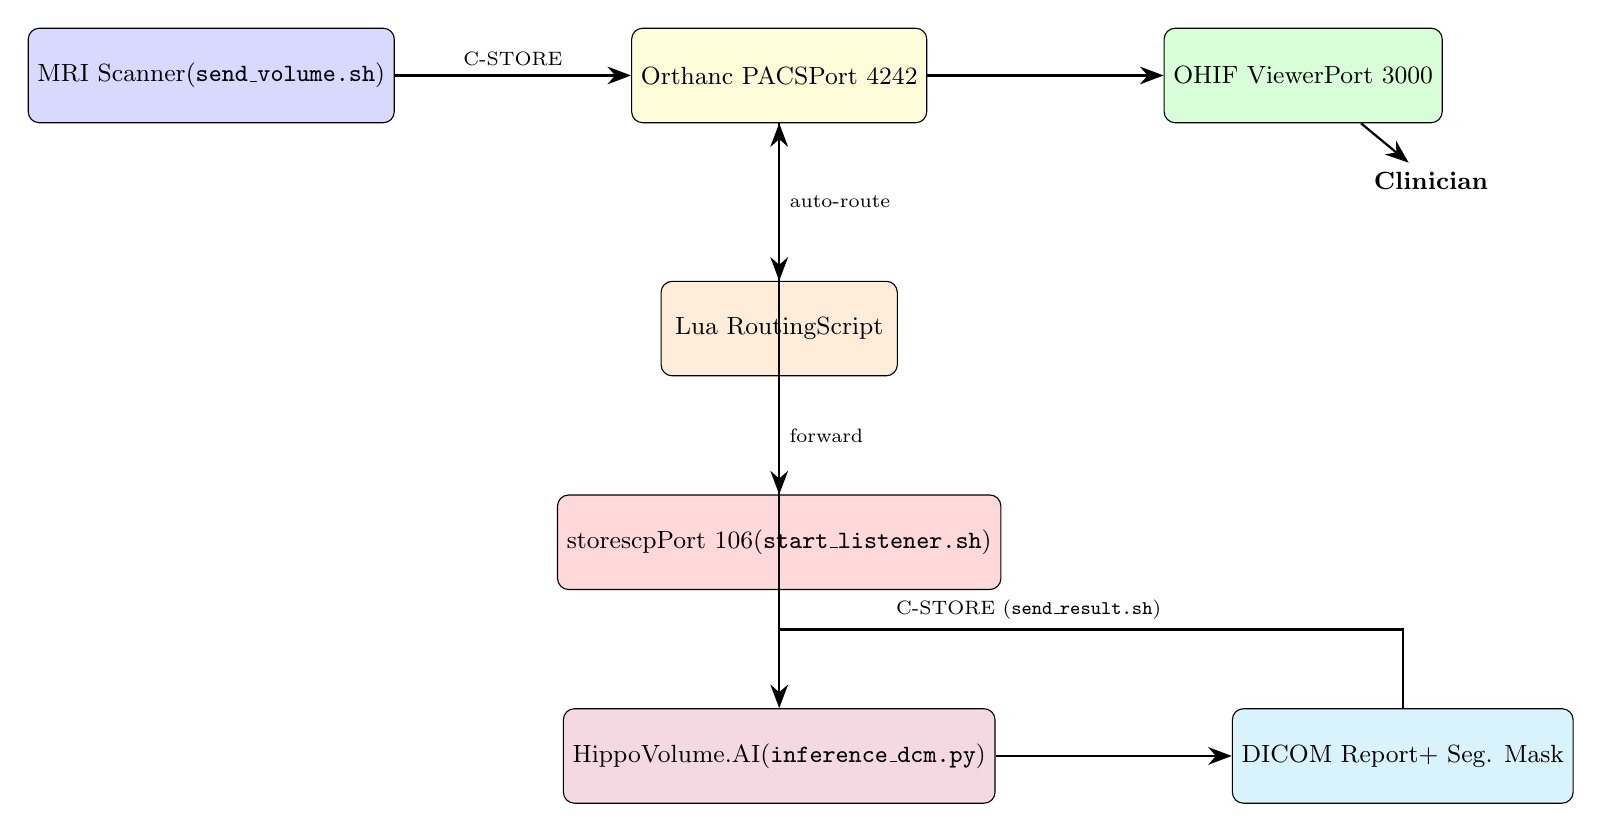
\begin{tikzpicture}[
    node distance=1.5cm and 3cm,
    box/.style={rectangle, draw, rounded corners, minimum width=3cm, minimum height=1.2cm, text centered, font=\small},
    arrow/.style={-{Stealth[length=3mm]}, thick},
]

% Nodes
\node[box, fill=blue!15] (scanner) {MRI Scanner\\(\texttt{send\_volume.sh})};
\node[box, fill=yellow!15, right=of scanner] (orthanc) {Orthanc PACS\\Port 4242};
\node[box, fill=green!15, right=of orthanc] (ohif) {OHIF Viewer\\Port 3000};

\node[box, fill=orange!15, below=2cm of orthanc] (lua) {Lua Routing\\Script};
\node[box, fill=red!15, below=of lua] (listener) {storescp\\Port 106\\(\texttt{start\_listener.sh})};
\node[box, fill=purple!15, below=of listener] (ai) {HippoVolume.AI\\(\texttt{inference\_dcm.py})};
\node[box, fill=cyan!15, right=of ai] (report) {DICOM Report\\+ Seg. Mask};

% Arrows
\draw[arrow] (scanner) -- node[above, font=\scriptsize] {C-STORE} (orthanc);
\draw[arrow] (orthanc) -- (ohif);
\draw[arrow] (orthanc) -- node[right, font=\scriptsize] {auto-route} (lua);
\draw[arrow] (lua) -- node[right, font=\scriptsize] {forward} (listener);
\draw[arrow] (listener) -- (ai);
\draw[arrow] (ai) -- (report);
\draw[arrow] (report.north) -- ++(0,1) -| node[above, font=\scriptsize, pos=0.3] {C-STORE (\texttt{send\_result.sh})} (orthanc.south);

% Clinician
\node[below right=0.5cm and -1cm of ohif, font=\small] (clin) {\textbf{Clinician}};
\draw[arrow] (ohif) -- (clin);

\end{tikzpicture}
\caption{Clinical deployment workflow. The MRI scanner sends images to PACS, which routes them to the AI system. Results are sent back and viewed by clinicians.}
\label{fig:clinical-deploy}
\end{figure}

\section{Deployment Scripts}

\subsection{route\_dicoms.lua}
The Orthanc auto-routing script. Runs inside the Orthanc PACS server:
\begin{lstlisting}[language={[5.0]Lua}]
function OnStoredInstance(instanceId, tags, metadata)
    SendToModality(instanceId, 'hippoai')
end
\end{lstlisting}
This tells Orthanc: ``Every time a new DICOM is stored, forward it to the modality named `hippoai'.''

\subsection{start\_listener.sh}
\begin{lstlisting}[language=bash]
# Upload routing script to Orthanc
curl -X POST http://localhost:8042/tools/execute-script \
     --data-binary @route_dicoms.lua -v

# Start DICOM listener
sudo storescp 106 -v -aet HIPPOAI \
     -od /path/to/route/dir \
     --sort-on-study-uid st
\end{lstlisting}

\subsection{send\_volume.sh}
\begin{lstlisting}[language=bash]
# Simulate MRI scanner sending a study to PACS
storescu 127.0.0.1 4242 -v -aec HIPPOAI \
         +r +sd /data/TestVolumes/Study1
\end{lstlisting}

\section{Series Selection (get\_series\_for\_inference)}

Not all MRI series are hippocampal crops. The function uses multi-criteria filtering:

\begin{enumerate}
    \item \textbf{Primary}: Look for \texttt{SeriesDescription} containing ``HippoCrop''
    \item \textbf{Fallback}: Group by \texttt{SeriesInstanceUID}, find series with small image dimensions ($< 100 \times 100$)
    \item \textbf{Validation}: Ensure exactly one matching series exists
    \item \textbf{Logging}: Print series metadata for audit trail
\end{enumerate}

\section{DICOM Volume Construction}

\begin{lstlisting}[language=Python, caption=Building 3D volume from DICOM slices]
def load_dicom_volume_as_numpy_from_list(dcmlist):
    slices = [np.flip(dcm.pixel_array).T 
              for dcm in sorted(dcmlist, key=lambda dcm: dcm.InstanceNumber)]
    hdr = dcmlist[0]
    hdr.PixelData = None
    return (np.stack(slices, 2), hdr)
\end{lstlisting}

\begin{itemize}
    \item Slices are sorted by \texttt{InstanceNumber} to ensure correct anatomical ordering
    \item \texttt{np.flip().T} corrects for DICOM's row-major patient orientation
    \item \texttt{np.stack(slices, 2)} assembles slices along the third axis
\end{itemize}

\section{DICOM Report Generation}

The \texttt{create\_report} function generates a comprehensive $1000 \times 1000$ RGB image:

\begin{enumerate}
    \item \textbf{Header}: ``HippoVolume.AI'' title
    \item \textbf{Patient Info}: ID, name, study date, modality, institution
    \item \textbf{Measurements}: Anterior, posterior, and total volumes in mm\textsuperscript{3} with percentages
    \item \textbf{Clinical Assessment}: Compares against reference range (2,500--4,500 mm\textsuperscript{3})
    \begin{itemize}
        \item Below range: \textcolor{red}{``BELOW normal range''} (red)
        \item Within range: \textcolor{green}{``Within normal reference range''} (green)
        \item Above range: \textcolor{orange}{``ABOVE normal range''} (orange)
    \end{itemize}
    \item \textbf{Visualizations}: Three axial slices with segmentation overlays
    \begin{itemize}
        \item \textcolor{green}{Green} = Anterior hippocampus
        \item \textcolor{red}{Red} = Posterior hippocampus
    \end{itemize}
    \item \textbf{Quality Metric}: Segmentation coverage (percentage of voxels segmented)
    \item \textbf{Disclaimer}: AI-generated report notice with model info
\end{enumerate}

\section{DICOM Secondary Capture Storage}

The report image is packaged as a \textbf{DICOM Secondary Capture (SC) Image} per DICOM PS3.3 Section A.8:

\begin{table}[H]
\centering
\small
\begin{tabular}{lll}
\toprule
\textbf{Module} & \textbf{Required} & \textbf{Our Implementation} \\
\midrule
Patient & Mandatory & Copied from original study \\
General Study & Mandatory & Study UID from original; fresh date/time \\
General Series & Mandatory & New Series UID; Series\# 9999 \\
General Equipment & Mandatory & ``HippoVolume.AI'' manufacturer \\
SC Equipment & Mandatory & Conversion type = WSD (workstation) \\
General Image & Mandatory & Instance\# 1; type DERIVED/PRIMARY \\
Image Pixel & Mandatory & RGB, 8-bit, $1000 \times 1000$ \\
SOP Common & Mandatory & SC Image Storage SOP Class \\
\bottomrule
\end{tabular}
\caption{DICOM modules included in the report}
\end{table}

\section{Stand-Out: Segmentation Mask DICOM Series}

Beyond the report, a separate DICOM series is created containing the actual segmentation mask:
\begin{itemize}
    \item One DICOM file per slice (matching the original volume)
    \item RGB color-coded: green (anterior), red (posterior)
    \item Proper \texttt{FrameOfReferenceUID} for image fusion
    \item Can be loaded into 3D Slicer or Radiant DICOM viewer for overlay visualization
\end{itemize}


% ============================================================
% CHAPTER 9: RESULTS AND ANALYSIS
% ============================================================
\chapter{Results and Analysis}

\section{Section 3 Output: Clinical Report}

The system generates a DICOM report (saved as \texttt{report.dcm} and \texttt{report.png}) containing:

\begin{itemize}
    \item Patient identification and study metadata
    \item Volumetric measurements with clinical context
    \item Three representative axial slice visualizations with segmentation overlays
    \item Clinical range assessment
    \item AI model information and disclaimer
\end{itemize}

The report image is located at \texttt{section3/out/report.png}. When running the full pipeline, this report is also stored as a DICOM Secondary Capture at \texttt{section3/out/report.dcm} and sent back to the PACS server.

\section{Performance Analysis}

\subsection{Best Performing Volumes}

\begin{table}[H]
\centering
\begin{tabular}{lcc}
\toprule
\textbf{Volume} & \textbf{Dice} & \textbf{Jaccard} \\
\midrule
hippocampus\_146 & 0.9368 & 0.8811 \\
hippocampus\_034 & 0.9329 & 0.8742 \\
hippocampus\_175 & 0.9323 & 0.8731 \\
hippocampus\_207 & 0.9313 & 0.8714 \\
hippocampus\_152 & 0.9304 & 0.8698 \\
\bottomrule
\end{tabular}
\caption{Top 5 performing test volumes}
\end{table}

\subsection{Worst Performing Volumes}

\begin{table}[H]
\centering
\begin{tabular}{lcc}
\toprule
\textbf{Volume} & \textbf{Dice} & \textbf{Jaccard} \\
\midrule
hippocampus\_334 & 0.8229 & 0.6991 \\
hippocampus\_305 & 0.8258 & 0.7032 \\
hippocampus\_125 & 0.8270 & 0.7050 \\
hippocampus\_042 & 0.8321 & 0.7124 \\
hippocampus\_070 & 0.8584 & 0.7519 \\
\bottomrule
\end{tabular}
\caption{Bottom 5 performing test volumes}
\end{table}

\subsection{Reasons for Performance Variation}
\begin{itemize}
    \item \textbf{Best volumes}: Clear hippocampal boundaries, larger hippocampal size, high SNR
    \item \textbf{Worst volumes}: Smaller hippocampi, ambiguous anterior-posterior boundaries, potential motion artifacts, anatomical variants
    \item The narrow spread (0.82--0.94) indicates robust overall performance
\end{itemize}


% ============================================================
% CHAPTER 10: STAND-OUT SUGGESTIONS IMPLEMENTED
% ============================================================
\chapter{Stand-Out Suggestions Implemented}

\section{Additional Evaluation Metrics}
\begin{itemize}
    \item \textbf{Sensitivity3d}: Measures under-segmentation risk
    \item \textbf{Specificity3d}: Measures over-segmentation risk
    \item \textbf{DicePerClass}: Separate Dice for anterior and posterior hippocampus
    \item Best/worst volume identification and tracking
\end{itemize}

\section{Single-Class Training Mode}
Command-line flag \texttt{--single-class} merges anterior and posterior labels:
\begin{lstlisting}[language=bash]
python run_ml_pipeline.py --single-class
\end{lstlisting}

\section{Enhanced Clinical Report}
\begin{itemize}
    \item Volume assessment against clinical reference range
    \item Color-coded alerts (red/green/orange)
    \item Segmentation quality indicator (coverage ratio)
    \item Model information and disclaimer
\end{itemize}

\section{Segmentation Mask DICOM Series}
Full DICOM series output for 3D visualization in clinical software.

\section{Multi-Criteria Series Selection}
Robust HippoCrop series identification with primary + fallback filtering strategies.

\section{Complete DICOM Compliance}
All mandatory modules per DICOM PS3.3 Section A.8 for Secondary Capture IOD.

\section{Training Report and Statistics}
Automated generation of training statistics, efficiency analysis, and suggestions.


% ============================================================
% CHAPTER 11: ENVIRONMENT & DEPENDENCIES
% ============================================================
\chapter{Environment and Dependencies}

\section{Section 2 Environment (GPU Training)}

\begin{table}[H]
\centering
\begin{tabular}{ll}
\toprule
\textbf{Package} & \textbf{Version} \\
\midrule
Python & 3.7 \\
PyTorch & 1.3.1 (CUDA 10.0) \\
cuDNN & 7.6.5 \\
nibabel & (NIFTI I/O) \\
medpy & (Medical image loading) \\
tensorboard & (Training monitoring) \\
numpy & (Array operations) \\
matplotlib & (Visualization) \\
\bottomrule
\end{tabular}
\end{table}

\section{Section 3 Environment (CPU Inference)}

\begin{table}[H]
\centering
\begin{tabular}{ll}
\toprule
\textbf{Package} & \textbf{Version} \\
\midrule
Python & 3.7 \\
PyTorch & 1.4.0 (CPU only) \\
pydicom & 1.4.2 \\
nibabel & 3.0.1 \\
Pillow & (Image generation) \\
numpy & (Array operations) \\
matplotlib & (Visualization) \\
scipy & (Scientific computing) \\
\bottomrule
\end{tabular}
\end{table}

\begin{infobox}{Why CPU-Only for Section 3?}
Clinical deployment environments typically don't have GPUs. The model is small enough that CPU inference on a single volume takes $<5$ seconds, which is clinically acceptable. This also simplifies deployment and reduces infrastructure costs.
\end{infobox}


% ============================================================
% CHAPTER 12: KEY CONCEPTS GLOSSARY
% ============================================================
\chapter{Key Concepts Glossary}

\begin{description}[style=nextline]
    \item[Alzheimer's Disease] Progressive neurodegenerative disorder causing memory loss and cognitive decline. Hippocampal atrophy is an early biomarker.
    
    \item[Axial Slice] A horizontal cross-section of the brain, as if looking from above. This is the slicing direction used in our 2D U-Net.
    
    \item[C-STORE] A DICOM network command for sending (``storing'') images to a PACS server.
    
    \item[Cross-Entropy Loss] Loss function that measures the difference between predicted class probabilities and true labels. Standard for classification/segmentation.
    
    \item[DICOM] Digital Imaging and Communications in Medicine. Universal standard for medical image storage and transmission.
    
    \item[Dice Coefficient] Overlap metric: $\frac{2|A \cap B|}{|A| + |B|}$. Values near 1.0 indicate good segmentation.
    
    \item[Hippocampus] Brain structure in the medial temporal lobe crucial for memory formation.
    
    \item[Instance Normalization] Normalizes each feature map of each sample independently. Better than Batch Norm for small batches.
    
    \item[Jaccard Index] IoU metric: $\frac{|A \cap B|}{|A \cup B|}$. More intuitive than Dice.
    
    \item[NIFTI] Neuroimaging file format storing 3D volumes in a single file. Used in research.
    
    \item[OHIF] Open Health Imaging Foundation. Web-based DICOM viewer.
    
    \item[Orthanc] Open-source, lightweight PACS server.
    
    \item[PACS] Picture Archiving and Communication System. Hospital image storage infrastructure.
    
    \item[Secondary Capture] A DICOM IOD type for non-acquisition images (reports, screenshots, AI results).
    
    \item[Segmentation] The task of assigning a class label to every pixel/voxel in an image.
    
    \item[Skip Connection] Direct pathway between encoder and decoder in U-Net that preserves spatial detail.
    
    \item[Softmax] Function that converts raw logits to probabilities: $\sigma(z_i) = \frac{e^{z_i}}{\sum_j e^{z_j}}$.
    
    \item[storescp/storescu] DCMTK command-line tools for receiving (SCP) and sending (SCU) DICOM files.
    
    \item[U-Net] Encoder-decoder CNN architecture with skip connections, designed for biomedical image segmentation.
    
    \item[Voxel] A 3D pixel. In our dataset, each voxel represents $1 \times 1 \times 1$ mm\textsuperscript{3} of brain tissue.
\end{description}


\end{document}
